%%%%%%%%%%%%%%%%%%%%%%%%%%%%%%%%%%%%%%%%%%%%%%%%%%%%%%%%%%%%%%%%%%%%%%%%%%%%%%%%%%%
%% This project aims to create the UNAL template for presentation.               %%
%% author:Félix Julián Gutiérrez                                                 %%
%% contacts:                                                                     %%
%%    e-mail: fjgutierrezb@unal.edu.co                                           %%
%%   www.unal.edu.co                                                             %%
%%%%%%%%%%%%%%%%%%%%%%%%%%%%%%%%%%%%%%%%%%%%%%%%%%%%%%%%%%%%%%%%%%%%%%%%%%%%%%%%%%%
\documentclass{libs/ufc_format}
% Inserting the preamble file with the packages
%%%%%%%%%%%%%%%%%%%%%%%%%%%%%%%%%%%%%%%%%%%%%%%%%%%%%%%%%%%%%%%%%%%%%
%% This file contains the packages that can be used in the beamer. %%
%%%%%%%%%%%%%%%%%%%%%%%%%%%%%%%%%%%%%%%%%%%%%%%%%%%%%%%%%%%%%%%%%%%%%
% Package to fonts family
\usepackage[T1]{fontenc}
% Package to accentuation
\usepackage[utf8]{inputenc}
% Package to Spanish language
\usepackage[spanish]{babel}
% Package to Figures
\usepackage{graphicx}
% Package to the colors
\usepackage{color}
% Package to the colors
\usepackage{xcolor}
% Packages to math symbols and expressions
\usepackage{amsfonts, amssymb, amsmath}
% Package to multiple lines and columns in table
\usepackage{multirow, array} 
% Package to create pseudo-code
% For more detail of this package: http://linorg.usp.br/CTAN/macros/latex/contrib/algorithm2e/doc/algorithm2e.pdf
\usepackage{algorithm2e}
% Package to insert code
\usepackage{listings} 
\usepackage{keyval}
% Package to justify text
\usepackage[document]{ragged2e}
% Package to manage the bibliography
\usepackage[backend=biber, style=numeric, sorting=none]{biblatex}
% Package to facilities quotations
\usepackage{csquotes}
% Package to use multicols
\usepackage{multicol}

% SVG (CUSTOM)
\usepackage{svg}
% Inserting the references file
\bibliography{references.bib}

% Title
\title[Sistemas Operativos]{\huge\textbf{}}
% Subtitle
\subtitle{\textbf{El Sistema Operativo XV6 - Capítulo 3 - Parte 1}}
% Author of the presentation
\author{Carlos Santiago Sandoval Casallas}
% Institute's Name
\institute[UNAL]{
    % email for contact
    \normalsize{\email{csandovalc@unal.edu.co}}
    \newline
    % Department Name
    \department{Departamento de Ingeniería de Sistemas e Industrial}
    \newline
    % university name
    \ufc
}
% date of the presentation
\date{\today}

%%%%%%%%%%%%%%%%%%%%%%%%%%%%%%%%%%%%%%%%%%%%%%%%%%%%%%%%%%%%%%%%%%%%%%%%%%%%%%%%%%
%% Start Document of the Presentation                                           %%               
%%%%%%%%%%%%%%%%%%%%%%%%%%%%%%%%%%%%%%%%%%%%%%%%%%%%%%%%%%%%%%%%%%%%%%%%%%%%%%%%%%
\begin{document}
% insert the code style
%%%%%%%%%%%%%%%%%%%%%%%%%%%%%%%%%%%%%%%%%%%%%%%%%%%%%%%%%%%%%%%%%%%%%%%%%%%%%%%%%%%
%% This file contains the style of the codes show in slides.                     %%
%% The package used is listings, but it possible to used others.                 %%
%%%%%%%%%%%%%%%%%%%%%%%%%%%%%%%%%%%%%%%%%%%%%%%%%%%%%%%%%%%%%%%%%%%%%%%%%%%%%%%%%%%

% color used in the code style
\definecolor{codegreen}{rgb}{0,0.6,0}
\definecolor{codegray}{rgb}{0.5,0.5,0.5}
\definecolor{codepurple}{rgb}{0.58,0,0.82}
\definecolor{codebackground}{rgb}{0.95,0.95,0.92}

% style of the code!
\lstdefinestyle{codestyle}{
    backgroundcolor=\color{codebackground},   
    commentstyle=\color{codegreen},
    keywordstyle=\color{magenta},
    numberstyle=\tiny\color{codegray},
    stringstyle=\color{codepurple},
    basicstyle=\ttfamily\footnotesize,
    frame=single,
    breakatwhitespace=false,         
    breaklines=true,                 
    captionpos=b,                    
    keepspaces=true,                 
    numbers=left,                    
    numbersep=5pt,                  
    showspaces=false,                
    showstringspaces=false,
    showtabs=false,                  
    tabsize=2,
    title=\lstname 
}

\lstset{style=codestyle}


%% ---------------------------------------------------------------------------
% First frame (with tile, subtitle, ...)
\begin{frame}
    \maketitle
\end{frame}

%% ---------------------------------------------------------------------------
% Second frame
\begin{frame}{Agenda}
    % \begin{multicols}{2}
        \tableofcontents
    % \end{multicols}
\end{frame}
%% ---------------------------------------------------------------------------
\section{Tablas de páginas}
\begin{frame}{Descripción}
    Anteriormente se trató el aislamiento y la importancia de brindar al proceso la ilusión de un espacio de direcciones y memoria único. Las tablas de páginas son el mecanismo más empleado por los sistemas operativos para cumplir con este objetivo \cite{xv6_book}, estas determinan el significado de las direcciones de memoria y las partes de la memoria física que son accesibles.

    \vspace{0.3cm}

    Esta estrategia es ampliamente usada, esto debido, a que permite llevar a cabos “trucos” con la memoria, por ejemplo, asignar la misma página de trampolín en varios espacios de direcciones, proteger las pilas de kernel y del usuario mediante páginas sin asignar, esto último, con el fin de evitar que en caso de un desbordamiento de la memoria las pilas sean sobreescritas.
\end{frame}
%% ---------------------------------------------------------------------------
\section{Hardware de paginación}
\begin{frame}{Hardware de paginación}
    Se destaca que: \emph{las instrucciones de RISC-V manipula las direcciones virtuales}. La memoria física es indexada a través de \emph{direcciones físicas}, el hardware de la tabla de páginas que brinda RISC-V se encarga de conectar estos dos tipos de direcciones, asignando cada dirección virtual a una dirección física.

    \vspace{0.3cm}

    XV6 se ejecuta sobre un Sv39 RISC-V, esto indica que solo se emplean los 39 bits menos significativos de una dirección virtual de 64 bits, los 25 bits restantes no se utilizan.
\end{frame}
%% ---------------------------------------------------------------------------
\begin{frame}{}
     Una tabla de páginas \example{(figura \ref{fig:tabla_paginas_lineal})} es una matriz con $2^{27}$ entradas, estas reciben el nombre de PTE (\textbf{P}age \textbf{T}able \textbf{E}ntry). Cada PTE contiene un número de página física o PPN (\textbf{P}hysical \textbf{P}age \textbf{N}umber) de 44 bits, además, se emplean 10 bits adicionales para algunos indicadores. 


    \vspace{0.3cm}
    
    El hardware de paginación traduce una dirección virtual, emplea 27 bits, \emph{los más significativos}, de los 39 disponibles, estos bits permiten indexar cada PTE, del cual se extrae el PPN almacenado, los 44 bits del PPN serán los 44 bits más significativos de una dirección física de 56 bits, donde los 12 bits restantes son extraídos de los bits menos significativos de la dirección virtual original.

    \begin{block}{Que es una página?}
        En XV6 se define una página como un segmento de memoria alineado, cuyo tamaño es de $2^{12}$ (4096) bytes. \cite{xv6_book}
    \end{block}
\end{frame}
%% ---------------------------------------------------------------------------
\begin{frame}{}
    \begin{figure}
        \centering
        \caption{Sistema de direcciones virtuales y físicas de RISC-V, con una tabla simplificada. \cite{xv6_book}}
        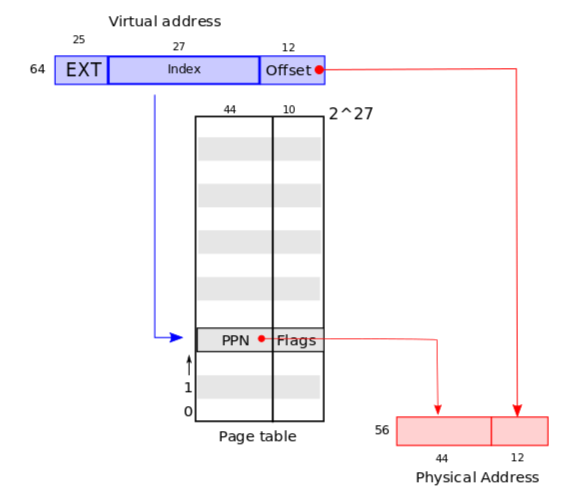
\includegraphics[scale=0.35]{libs/img/riscv_address.png}
        \source{xv6: a simple, Unix-like teaching operating system \cite{xv6_book}}
        \label{fig:tabla_paginas_lineal}
    \end{figure}
\end{frame}

%% ---------------------------------------------------------------------------
\begin{frame}{}
    En Sv39 RISV-V, los 25 bits superiores \emph{no se utilizan para la traducción}. Por su parte, la dirección física tiene espacio para crecer, dado que el PTE emplea 54 de los 64 bits disponibles, \example{44 para el PPN y 10 para los indicadores}, por lo que puede crecer estos 10 bits, esta fue una decisión de los diseñadores de RISC-V con base en el futuro.

    \vspace{0.3cm}

    Si consideramos el sistema lineal ya mostrado, se pueden representar un total de $2^{39}$ bytes en la memoria virtual, lo que sería aproximadamente 512 GB, esto se considera como suficiente espacio para que las aplicaciones se puedan ejecutar sobre la computadora RISC-V, por su parte, se pueden representar $2^{56}$ bytes en la memoria física, permite al sistema abordar y adaptar múltiples dispositivos. \cite{xv6_book} \newline
    \example{En caso de que se requiera de mas capacidad, ya se ha definido Sv48, el cual posee direcciones virtuales de 48 bits. \cite{xv6_book}}
\end{frame}
%% ---------------------------------------------------------------------------
\begin{frame}{Traducción en tres pasos}
    \begin{figure}
        \centering
        \caption{Sistema de traducción de direcciones. \cite{xv6_book}}
        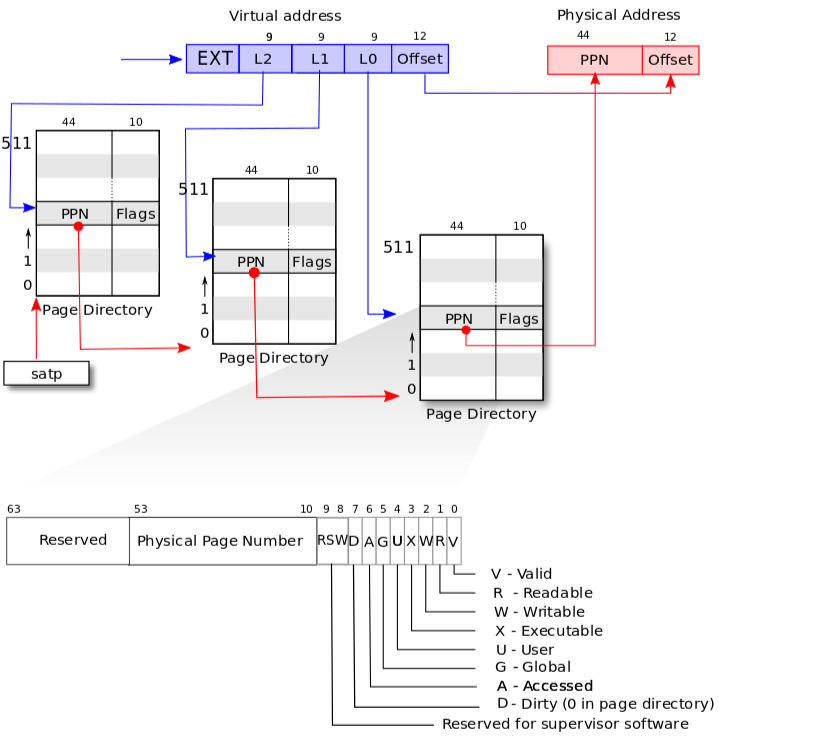
\includegraphics[scale=0.23]{libs/img/riscv_pagetable.png}
        \source{xv6: a simple, Unix-like teaching operating system \cite{xv6_book}}
        \label{fig:sistema_arbol}
    \end{figure}
\end{frame}
%% ---------------------------------------------------------------------------
\begin{frame}{}
    Una CPU RISC-V traduce una dirección virtual a una física en tres pasos. La tabla de páginas se almacena en la memoria física como un \emph{árbol de tres niveles de profundidad}.

    \vspace{0.2cm}
    
    La raíz del árbol es una tabla de páginas de 4096 bytes que contiene 512 PTE de 64 bits cada uno, cada PTE contiene la dirección física de la tabla de páginas del siguiente nivel del árbol, el nivel más profundo del árbol, contiene los 44 bits superiores de la dirección física a la que se hace referencia, los 12 bits restantes provienen de los 12 bits menos significativos de la dirección virtual original. \cite{xv6_book}
\end{frame}
%% ---------------------------------------------------------------------------
\begin{frame}{}
     El hardware de paginación utiliza los 9 bits superiores de los 27 bits más significativos \emph{(de los 39 utilizables)} para indexar un PTE en la tabla de páginas raíz, cuya dirección física es almacenada en el registro \emph{satp}, los siguientes 9 para un PTE del nivel medio y los 9 inferiores para indexar un PTE del nivel final del árbol. \cite{xv6_book}

     \vspace{0.4cm}

    \begin{block}{Sistema en Sv48}
        En Sv48 RISC-V, una tabla de páginas tiene cuatro niveles y los bits 39 al 47 indexan las direcciones virtuales en el nivel más alto. \cite{xv6_book}
    \end{block}
\end{frame}
%% ---------------------------------------------------------------------------
\begin{frame}{Fallo de página}
    Si alguno de los tres PTE's necesarios para traducir una dirección no está presente, el hardware de paginación lanza una excepción de fallo de página, dejando que el kernel maneje la situación (se profundizara en el capítulo 4 del libro). \cite{xv6_book}

    \vspace{0.3cm}

    El sistema propuesto en la figura \ref{fig:sistema_arbol}, permite manejar direcciones virtuales con alta eficiencia de la memoria, en comparación con el sistema línea de la figura \ref{fig:tabla_paginas_lineal}. En el caso de que grandes rangos de direcciones virtuales no tengan una asignación, la estructura de tres niveles puede omitir directorios de página completos.
\end{frame}
%% ---------------------------------------------------------------------------
\begin{frame}{}
    Esto quiere decir que si una aplicación usa pocas páginas y estas empiezan desde la dirección cero, en el directorio raíz, las entradas de la 1 a la 511 del directorio de páginas de nivel superior no son válidas, \emph{y el kernel no tiene que asignar directorios a sus páginas intermedias} y a su vez \emph{no requieren de los directorios del nivel más bajo para cada uno de esos 511 directorios intermedios}, por lo que este sistema puede ahorrar 511 páginas intermedias y 511 * 512 páginas de directorios del nivel más profundo.\newline

    \vspace{0.2cm}
    
    A diferencia del sistema lineal, donde dicha optimización no es posible. \cite{xv6_book}
\end{frame}
%% ---------------------------------------------------------------------------
\begin{frame}{Desventajas del sistema de árbol}
    Cuando una CPU ejecuta una instrucción de carga o almacenamiento, es necesario que la CPU recorra toda la estructura, \emph{y el sistema debe cargar tres entradas del sistema de árbol} desde la memoria para realizar la traducción de la dirección virtual para ejecutar la instrucción de carga/almacenamiento sobre una dirección física. Para evitar este costo adicional de cargar un PTE desde la memoria física, la CPU puede almacenar en caché las entradas de la tabla de páginas en un búfer, conocido como TLB (\textbf{T}ranslation \textbf{L}ook-aside \textbf{B}uffer). \cite{xv6_book}
\end{frame}
%% ---------------------------------------------------------------------------
\begin{frame}{Sistema de banderas o indicadores}
    Cada PTE contiene unos bits indicadores, que definen el comportamiento permitido para el hardware sobre la dirección virtual asociada, estas banderas están en la figura \ref{fig:sistema_arbol} y se profundiza en la lista:

    \vspace{0.2cm}
    
    \begin{itemize}
        \item \textbf{PTE\_V:} Indica si el PTE está presente, en caso de que no lo esté, el hacer referencia a esta página provocará una excepción dado que no está permitido su acceso.
        \item \textbf{PTE\_R:} Controla si las instrucciones pueden leer en la página.
        \item \textbf{PTE\_W:} Controla si las instrucciones pueden escribir en la página.
        \item \textbf{PTE\_X:} Controla si la CPU puede interpretar el contenido de la página como instrucciones a ejecutar.
    \end{itemize}
\end{frame}
%% ---------------------------------------------------------------------------
\begin{frame}{}
    \begin{itemize}
        \item \textbf{PTE\_U:} Controla si las instrucciones ejecutadas en modo usuario pueden acceder a la página, en caso de que este atributo no este configurado, el PTE solo puede ser empleado en modo supervisor (kernel).
    \end{itemize}

    \vspace{0.3cm}

    Las banderas y las estructuras relacionadas se encuentran en: \href{https://github.com/CarlosSandoval-03/xv6-riscv/blob/riscv/kernel/riscv.h}{\textbf{\textit{(kernel/riscv.h)}}} \cite{xv6_book} \cite{xv6}
\end{frame}
%% ---------------------------------------------------------------------------
\begin{frame}{Uso de la tabla de páginas}
    Para que una CPU use una tabla de páginas, el kernel debe escribir la dirección física de la página que contiene la tabla de páginas raíz en el registro \textbf{satp}. Una CPU se encargará de traducir todas las direcciones generadas por instrucciones posteriores empleando la tabla a la que apunta su propio \textbf{satp}. \cite{xv6_book}
    
    \vspace{0.3cm}
    
    \emph{Cada CPU tiene su propio satp}, para que diferentes CPU puedan ejecutar diferentes procesos, cada uno con su espacio de direcciones privado, el cual es descrito por la tabla de páginas referenciada. \cite{xv6_book}
\end{frame}
%% ---------------------------------------------------------------------------
\begin{frame}{Administración de memoria del kernel}
    El kernel \emph{mapea toda la memoria física en su propia página de tablas}, esto le permite leer y escribir en cualquier ubicación de la memoria física empleando las instrucciones de carga y almacenamiento. Dado que tiene acceso a todos los directorios de páginas, el kernel puede alterar el contenido de un PTE de un directorio de páginas escribiendo en la dirección virtual del PTE mediante instrucciones de almacenamiento estándar. \emph{En resumen, puede alterar el valor de un PTE escribiendo directamente sobre él. \cite{xv6_book}}
\end{frame}
%% ---------------------------------------------------------------------------
\begin{frame}{Revisión de conceptos}
    Cuando se habla de memoria física, se hace referencia a las celdas de almacenamiento en DRAM. Un byte de memoria física tiene una dirección, esta se llama dirección física. \emph{Las instrucciones solo usan direcciones virtuales}, que es traducida a direcciones físicas por el hardware de paginación y \emph{luego es enviado al hardware DRAM} para leer o escribir en la unidad de almacenamiento.
    
    \vspace{0.3cm}

    A diferencia de la memoria física y las direcciones virtuales, la memoria virtual no es un objeto físico, sino más bien, un \emph{conjunto de abstracciones y mecanismos} que emplea el kernel para administrar memoria física y direcciones virtuales. \cite{xv6_book}
\end{frame}
%% ---------------------------------------------------------------------------
\section{Espacio de direcciones}
\begin{frame}{Disposición de memoria en XV6}
    \begin{figure}
        \centering
        \caption{Izq: El espacio de direcciones del kernel, Der:Espacio de direcciones físicas de RISC-V \cite{xv6_book}}
        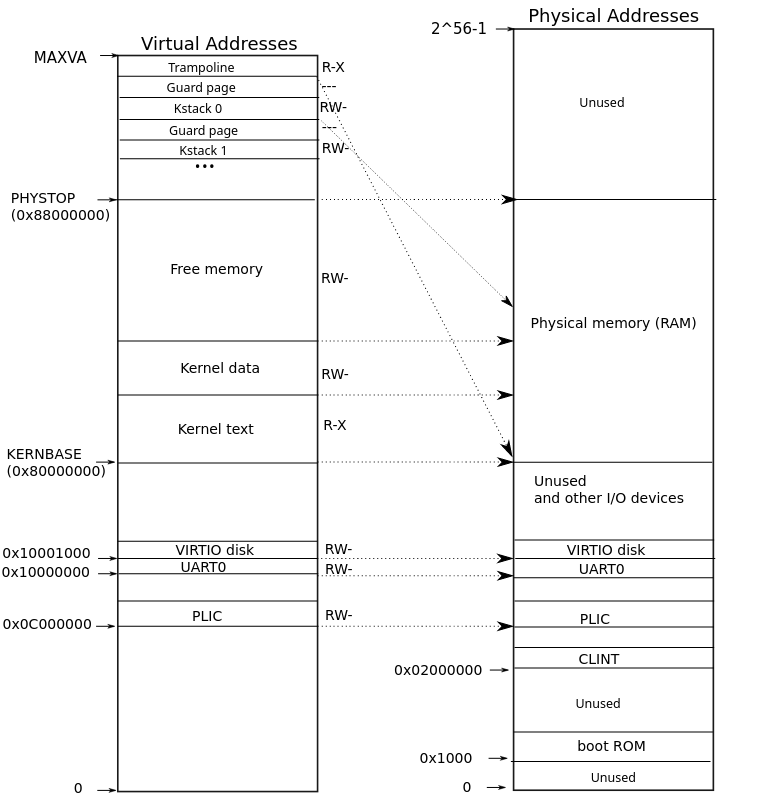
\includegraphics[scale=0.2]{libs/img/xv6_layout.png}
        \source{xv6: a simple, Unix-like teaching operating system \cite{xv6_book}}
        \label{fig:esquema_dir_kernel}
    \end{figure}
\end{frame}
%% ---------------------------------------------------------------------------
\begin{frame}{Espacio de direcciones del kernel}
    XV6 emplea una tabla de páginas por proceso, esta tabla describe el espacio de direcciones de usuario de cada proceso, pero adicionalmente, implementa una tabla de una \emph{única página} que describe el espacio de direcciones del kernel.
    
    \vspace{0.3cm}
    
    El kernel configura su propio espacio de direcciones para poder acceder a la memoria física y los recursos de hardware en direcciones virtuales predecibles, esta disposición se puede apreciar en la figura \ref{fig:esquema_dir_kernel} y en el archivo \href{https://github.com/CarlosSandoval-03/xv6-riscv/blob/riscv/kernel/memlayout.h}{\textbf{\textit{(kernel/memlayout.h)}}} \cite{xv6}, este último es donde se declaran las constantes para el diseño de la memoria del kernel de XV6. \cite{xv6_book}
\end{frame}
%% ---------------------------------------------------------------------------
\begin{frame}{QEMU}
    QEMU simula una computadora que incluye RAM, la cual comienza en la dirección física \textbf{0x80000000} y continua hasta al menos la dirección \textbf{0x88000000}, esta última recibe el nombre de \example{PHYSTOP}. Adicionalmente, QEMU también simula dispositivos de E/S, \example{por ej. una interfaz de disco}. QEMU expone al software las interfaces de los dispositivos como registros de control asignados por debajo de la dirección física \textbf{0x80000000}.

    \vspace{0.3cm}

    El kernel puede interactuar con los dispositivos leyendo/escribiendo estas direcciones físicas especiales, las operaciones sobre estas direcciones se ejecutan directamente en el hardware del dispositivo en vez de la RAM. \cite{xv6_book}
\end{frame}
%% ---------------------------------------------------------------------------
\begin{frame}{}
    El kernel accede a la RAM y a los registros de dispositivos que son mapeados en memoria usando el mapeo directo; es decir, que \emph{la dirección virtual es igual a la dirección física}. Un ejemplo evidente es la ubicación del kernel, este se encuentra en \textbf{KERNBASE} o \textbf{(0x80000000)}, esto tanto en la dirección virtual como en la memoria física. Esta implementación \emph{simplifica el código del kernel} cuando es necesario leer o escribir en la memoria física. \cite{xv6_book}.
    
    \vspace{0.3cm}
    
    Sin embargo, este método no es aplicado por el kernel en su totalidad, existen direcciones virtuales las cuales no están asignadas directamente.
\end{frame}
%% ---------------------------------------------------------------------------
\begin{frame}{Asignaciones no directas del kernel}
    Estas direcciones virtuales no asignadas directamente son:
    \begin{itemize}
        \item \textbf{La página del trampolín:} Esta página es asignada en la parte superior del espacio de direcciones virtuales, al igual que las direcciones altas de las tablas de página de usuario. La página que contiene el código del trampolín, es mapeada dos veces en las direcciones virtuales, una mediante mapeo directo \emph{(dado que esta se encuentra dentro del código del kernel)} y otra en las direcciones más altas de las direcciones virtuales. \cite{xv6_book}
    \end{itemize}
\end{frame}
%% ---------------------------------------------------------------------------
\begin{frame}{}
    \begin{itemize}
        \item \textbf{La página de la pila del kernel:} Cada proceso tiene su propia pila del kernel, esta se encuentra mapeada en direcciones altas y con una página de protección debajo de esta, la página de protección no tiene un PTE válido, es decir el indicador \textbf{PTE\_V} no está establecido, por lo que si la pila se desborda, provocará que el kernel entre en pánico. \emph{Es mejor generar un estado de pánico al kernel, que correr el riesgo de que el desbordamiento de pila pueda sobrescribir otras direcciones de memoria}. \cite{xv6_book}
    \end{itemize}

    \vspace{0.2cm}

    Aunque el kernel asigna sus pilas a las direcciones de memoria altas, estas también pueden ser accedidas por el kernel a través del mapeo directo.
\end{frame}
%% ---------------------------------------------------------------------------
\begin{frame}{Permisos asignados durante el mapeo}
    El kernel asigna a las páginas trampolín y el código del kernel los permisos de \textbf{PTE\_R} y\textbf{ PTE\_X}. El kernel lee y ejecuta las instrucciones desde estas páginas. Mientras que las otras páginas son mapeadas con los permisos \textbf{PTE\_R} y \textbf{PTE\_W}, para que el kernel pueda leer y escribir en la memoria de las páginas mapeadas, \emph{exceptuando las páginas de protección, las cuales no son páginas válidas}. \cite{xv6_book}
\end{frame}
%% ---------------------------------------------------------------------------
\section{Creando un espacio de direcciones}
\begin{frame}{Creando un espacio de direcciones}
    Gran parte del código para manipular espacio de direcciones y tablas de páginas se encuentra en \href{https://github.com/CarlosSandoval-03/xv6-riscv/blob/riscv/kernel/vm.c}{\textbf{\textit{(kernel/vm.c)}}}. Allí se define la estructura de datos principal \emph{pagetable\_t}, esta en realidad es un puntero a la raíz de una página la cual contiene una tabla de páginas de RISC-V, esta estructura puede representar una tabla de páginas del kernel o de un proceso.

    \vspace{0.4cm}

    Las funciones principales son \href{https://github.com/CarlosSandoval-03/xv6-riscv/blob/riscv/kernel/vm.c\#L86}{\textbf{\textit{walk (kernel/vm.c:86)}}}, el cual retorna la dirección del PTE correspondiente a una dirección virtual, y \href{https://github.com/CarlosSandoval-03/xv6-riscv/blob/riscv/kernel/vm.c\#L143}{\textbf{\textit{mappages (kernel/vm.c:143)}}} el cual crea los PTE's para nuevos mapeos de una dirección física. \cite{xv6_book} \cite{xv6}
\end{frame}
%% ---------------------------------------------------------------------------
    \begin{frame}{Convenciones y algunas funciones}
    Las funciones que comienzan con \textbf{kvm} manipulan la tabla de páginas del kernel, mientras que las funciones que comienzan con \textbf{uvm} manipulan una tabla de páginas de usuario, en otro caso, las funciones pueden ser empleadas para ambos casos.

    \vspace{0.4cm}

    \href{https://github.com/CarlosSandoval-03/xv6-riscv/blob/riscv/kernel/vm.c\#L352}{\textbf{\textit{copyout}}} y \href{https://github.com/CarlosSandoval-03/xv6-riscv/blob/riscv/kernel/vm.c\#L377}{\textbf{\textit{copyin}}} permiten copiar datos hacia y desde direcciones virtuales de usuario proporcionadas como argumentos de llamada al sistema, estas funciones están en el archivo \href{https://github.com/CarlosSandoval-03/xv6-riscv/blob/riscv/kernel/vm.c}{\textbf{\textit{(kernel/vm.c)}}} porque necesitan traducir esas direcciones para encontrar la memoria física correspondiente. \cite{xv6_book} \cite{xv6}
\end{frame}
%% ---------------------------------------------------------------------------
\begin{frame}{Arranque del sistema de memoria}
    Al inicio del arranque del sistema, la función \href{https://github.com/CarlosSandoval-03/xv6-riscv/blob/riscv/kernel/main.c\#L20}{\textbf{\textit{main}}} llama a \href{https://github.com/CarlosSandoval-03/xv6-riscv/blob/riscv/kernel/vm.c\#L54}{\textbf{\textit{kvminit (kernel/vm:54)}}} para crear la tabla de páginas del kernel mediante la función \href{https://github.com/CarlosSandoval-03/xv6-riscv/blob/riscv/kernel/vm.c\#L20}{\textbf{\textit{kvmmake (kernel/vm.c:20)}}}, esta llamada ocurre antes de que XV6 habilite la paginación en el RISC-V, por lo que las direcciones hacen referencia directamente a la memoria física.

    \vspace{0.3cm}

    \href{https://github.com/CarlosSandoval-03/xv6-riscv/blob/riscv/kernel/vm.c\#L20}{\textbf{\textit{kvmmake}}} primero asigna una página en la memoria física, para almacenar la página raíz de la tabla de páginas. Luego llama a \href{https://github.com/CarlosSandoval-03/xv6-riscv/blob/riscv/kernel/vm.c\#L132}{\textbf{\textit{kvmmap}}} para instalar las traducciones que el kernel necesita, traducciones como: los datos e instrucciones del kernel, la memoria física hasta \textbf{PHYSTOP} y los rangos de memoria que representan dispositivos. \cite{xv6_book} \cite{xv6}
\end{frame}
%% ---------------------------------------------------------------------------
\begin{frame}{}
    \href{https://github.com/CarlosSandoval-03/xv6-riscv/blob/riscv/kernel/proc.c\#L33}{\textbf{\textit{proc\_mapstacks (kernel/proc.c:33)}}} asigna una pila de kernel para cada proceso, para esto, llama a \href{https://github.com/CarlosSandoval-03/xv6-riscv/blob/riscv/kernel/vm.c\#L132}{\textbf{\textit{kvmmap}}}, para mapear cada pila en la dirección virtual generada por \href{https://github.com/CarlosSandoval-03/xv6-riscv/blob/riscv/kernel/memlayout.h\#L56}{\textbf{\textit{KSTACK}}}, lo que deja espacio para las páginas de protección de pila no válidas.
    `
    \vspace{0.3cm}

    \href{https://github.com/CarlosSandoval-03/xv6-riscv/blob/riscv/kernel/vm.c\#L132}{\textbf{\textit{kvmmap}}} llama a \href{https://github.com/CarlosSandoval-03/xv6-riscv/blob/riscv/kernel/vm.c\#L143}{\textbf{\textit{mappages}}} para asignar en una tabla de páginas un rango de direcciones virtuales a un rango de direcciones físicas. Este proceso se realiza por separado para cada intervalo de página de las direcciones virtuales en el rango, para realizar el mapeo emplea \href{https://github.com/CarlosSandoval-03/xv6-riscv/blob/riscv/kernel/vm.c\#L86}{\textbf{\textit{walk}}}, con el fin de encontrar la dirección del PTE de dicha dirección, luego inicializa el PTE para contener el PPN y los permisos deseados (RXW) y este es marcado como válido (V) por defecto \href{https://github.com/CarlosSandoval-03/xv6-riscv/blob/riscv/kernel/vm.c\#L158}{\textbf{\textit{(kernel/vm.c:158)}}}. \cite{xv6_book} \cite{xv6}
\end{frame}
%% ---------------------------------------------------------------------------
\begin{frame}{Walk}
    \href{https://github.com/CarlosSandoval-03/xv6-riscv/blob/riscv/kernel/vm.c\#L86}{\textbf{\textit{walk (kernel/vm.c:86)}}} imita el comportamiento del hardware de paginación de RISC-V mientras busca el PTE en una dirección virtual (Figura \ref{fig:sistema_arbol}). La función recorre la tabla de páginas de tres niveles, empleando los bits de dirección virtual de cada nivel para encontrar el PTE de la tabla de páginas del siguiente nivel o de la página final \href{https://github.com/CarlosSandoval-03/xv6-riscv/blob/riscv/kernel/vm.c\#L92}{\textbf{\textit{(kernel/vm.c:92)}}}.

    \vspace{0.2cm}
    
    \emph{Si el PTE hallado no es válido}, la página solicitada no se ha asignado, con base en sí el argumento alloc es distinto de cero, walk podrá asignar una nueva página en la tabla de páginas y ubicar allí la dirección física del PTE. La función devuelve la dirección del PTE en la capa mas profunda del árbol \href{https://github.com/CarlosSandoval-03/xv6-riscv/blob/riscv/kernel/vm.c\#L102}{\textbf{\textit{(kernel/vm.c:102)}}}. \cite{xv6_book} \cite{xv6}
\end{frame}
%% ---------------------------------------------------------------------------
\begin{frame}{}
    El correcto funcionamiento del código anterior, depende de que la memoria física sea mapeada de forma directa en el espacio de direcciones virtuales del kernel.
    
    \vspace{0.2cm}
    
    Dado que a medida que walk desciende en el árbol, este extraerá la dirección \emph{(física)} de la tabla de páginas del siguiente nivel del árbol \href{https://github.com/CarlosSandoval-03/xv6-riscv/blob/riscv/kernel/vm.c\#L94}{\textbf{\textit{(kernel/vm.c:94)}}}, y luego usará dicha dirección física como una \emph{dirección virtual}, para buscar el PTE en el siguiente nivel \href{https://github.com/CarlosSandoval-03/xv6-riscv/blob/riscv/kernel/vm.c\#L92}{\textbf{\textit{(kernel/vm.c:92)}}}. \cite{xv6_book} \cite{xv6}
\end{frame}
%% ---------------------------------------------------------------------------
\begin{frame}{Instalación y caché}
    \href{https://github.com/CarlosSandoval-03/xv6-riscv/blob/riscv/kernel/main.c\#L20}{\textbf{\textit{main}}} llama a \href{https://github.com/CarlosSandoval-03/xv6-riscv/blob/riscv/kernel/vm.c\#L62}{\textbf{\textit{kvminithart (kernel/vm.c:62)}}} para que instale la tabla de páginas del kernel, esto a través de, escribir la dirección física de la página raíz de la tabla de páginas en el registro \textbf{satp}. Después de esto, la CPU podrá traducir direcciones usando la tabla de páginas del kernel. \cite{xv6_book} \cite{xv6} \newline
    \example{El sistema cuenta con paginación!!!}

    \vspace{0.3cm}

    Cada CPU almacena en caché las entradas de la tabla de páginas en un búfer de búsqueda de traducción (TLB), pero cuando XV6 cambia una tabla de páginas, \emph{se debe indicar a la CPU que invalide las entradas TLB almacenadas en caché}, esto debido a que, la TLB podría emplear un mapeo antiguo, que apunte a una página física que haya sido asignada a otro proceso, permitiendo que un proceso modifique la memoria de otro proceso. \cite{xv6_book} \cite{xv6}
\end{frame}
%% ---------------------------------------------------------------------------
\begin{frame}{}
    RISC-V tiene la instrucción \textbf{SFENCE.VMA}, la cual vacía el TLB de la CPU actual. XV6 ejecuta \textit{SFENCE.VMA} en \textbf{kvminithart} después de recargar el contenido del registro \textit{satp} y en el código trampolín, que cambia a una tabla de páginas de usuario antes de volver al espacio de usuario \href{https://github.com/CarlosSandoval-03/xv6-riscv/blob/riscv/kernel/trampoline.S\#L89}{\textbf{\textit{(kernel/trampoline.S:89)}}}. \cite{riscv:priv}

    \vspace{0.3cm}

    También es necesario ejecutar \textbf{SFENCE.VMA} antes de cambiar el registro \textit{satp}, para esperar que todas las instrucciones pendientes de carga y almacenamiento, esto garantiza que todas las actualizaciones pendientes se realicen sobre la tabla de páginas antigua y no sobre la nueva. \cite{xv6_book} \cite{xv6}
\end{frame}
%% ---------------------------------------------------------------------------
    \begin{frame}{Flush Parcial en RISC-V}
    Para evitar vaciar el TLB completo, las CPU RISC-V permiten identificadores del espacio de direcciones (ASID) \cite{xv6_book} \cite{riscv:priv}. Por lo que el kernel podría vaciar solo las entradas de TLB para un espacio de direcciones en particular. \newline
    \emph{XV6 no emplea esta característica}
\end{frame}
%% ---------------------------------------------------------------------------
\section{Asignación de memoria física}
\begin{frame}{Asignación y seguimiento de memoria física}
    El kernel debe asignar y liberar memoria física en tiempo de ejecución para: las tablas de páginas, la memoria de usuario, las pilas del kernel y los búfers de las tuberías, etc. Para esto, XV6 emplea la memoria física entre el \textbf{KERNBASE} y el \textbf{PHYSTOP} (Figura \ref{fig:esquema_dir_kernel}) para realizar estas asignaciones en tiempo de ejecución. \cite{xv6_book}

    \vspace{0.3cm}

    XV6 realiza un seguimiento de las páginas libres mediante el uso de una lista enlazada empleando las propias páginas libres. La asignación consiste en \emph{eliminar una página de la lista enlazada}, liberar consiste en \emph{agregar la página a la lista enlazada}. \cite{xv6_book}
\end{frame}
%% ---------------------------------------------------------------------------
% \section{Código: Asignador de memoria física}
% \section{Espacio de direcciones de un proceso}
% \section{Código: sbrk}
% \section{Código: exec}
% \section{Mundo real}

    % \begin{figure}
        % \centering
    %     \caption{Diseño del espacio de direcciones virtuales de un proceso}
    %     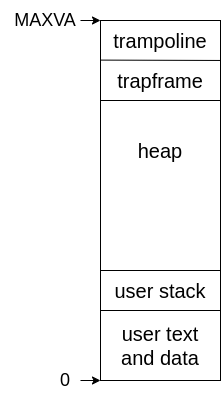
\includegraphics[scale=0.3]{libs/img/as.png}
    %     \source{xv6: a simple, Unix-like teaching operating system \cite{xv6_book}}
    %     \label{fig:Espacio_Direcciones}
    % \end{figure}

% %% ---------------------------------------------------------------------------
% \subsection{subsección 2}
% \begin{frame}{Bloques}
%     % Blocks styles
%     \begin{block}{Bloque azul}
%         fondo bloque en blanco.
%     \end{block}

%     \begin{alertblock}{Bloque de alerta}
%         fondo bloque en blanco.
%     \end{alertblock}

%     \begin{exampleblock}{Bloque de ejemplo}
%         fondo bloque en blanco..
%     \end{exampleblock}   
% \end{frame}

% %% ---------------------------------------------------------------------------
% \subsection{uso de cajas con enfasis}
% \begin{frame}{Para el uso con cajas, en especial programación}
%     \successbox{cajas de test}

%     \pause

%     \alertbox{Alerta de test}

%     \pause

%     \simplebox{Estado de test}
% \end{frame}

% %% ---------------------------------------------------------------------------
% \subsection{Algoritmos}
% \begin{frame}{para Algoritmos (Pseudocódigo)}
%     \begin{algorithm}[H]
%         \SetAlgoLined
%         \LinesNumbered
%         \SetKwInOut{Input}{input}
%         \SetKwInOut{Output}{output}
%         \Input{x: float, y: float}
%         \Output{r: float}
%         \While{True}{
%           r = x + y\;
%           \eIf{r >= 30}{
%            ``O valor de $r$ é maior ou iqual a 10.''\;
%            break\;
%            }{
%            ``O valor de $r$ = '', r\;
%           }
%          } 
%          \caption{Algorithm Example}
%     \end{algorithm}
% \end{frame}

% %% ---------------------------------------------------------------------------

% \begin{frame}{Insertando Algoritmos}
%     \lstset{language=Python}
%     \lstinputlisting[language=Python]{code/main.py}
% \end{frame}

% %% ---------------------------------------------------------------------------
% \begin{frame}{Insertando Algoritmos}
%     \lstinputlisting[language=C]{code/source.c}
% \end{frame}

% %% ---------------------------------------------------------------------------
% \begin{frame}{Insertando Algoritmos}
%     \lstinputlisting[language=Java]{code/helloworld.java}
% \end{frame}

% %% ---------------------------------------------------------------------------
% \begin{frame}{Insertando Algoritmos}
%     \lstinputlisting[language=HTML]{code/index.html}
% \end{frame}

% %% ---------------------------------------------------------------------------
% % This frame show an example to insert multicolumns
% \section{Sección II}
% \begin{frame}{Sección II}
%     \begin{columns}{}
%         \begin{column}{0.5\textwidth}
%             \justify
%            utilizado y justificado para 2 columnas
%         \end{column}
%         \begin{column}{0.5\textwidth}
%             \justify
%            espacioentre columnas para un segundo argumento
%         \end{column}
%     \end{columns}    
% \end{frame}

% %% ---------------------------------------------------------------------------
% % This frame show an example to insert figures
% \section{sección III}
% \begin{frame}{Sección III - Figuras}
%     \begin{figure}
%         \centering
%         \caption{logo UNAL.}
%         
\includegraphics[scale=0.3]{libs/UNAL_logo.jpg}
%         \source{Obtenido del sitio oficial \cite{xv6} \cite{xv6_book}}
%         \label{fig:Logo UNAL}
%     \end{figure}
% \end{frame}

%% ---------------------------------------------------------------------------
% Reference frames
\begin{frame}[allowframebreaks]
    \frametitle{Referencias}
    \printbibliography
\end{frame}

%% ---------------------------------------------------------------------------
% Final frame
\begin{frame}
    \centering
    \huge{\textbf{\example{Gracias por la atención}}}
    
    \vspace{1cm}
    
    \Large{\textbf{Contacto:}}
    \newline
    \vspace*{0.5cm}
    \large{\email{csandovalc@unal.edu.co}}
\end{frame}

\end{document}